%!TEX TS-program = xelatex
\documentclass[]{friggeri-cv}
\usepackage{afterpage}
\usepackage{hyperref}
\usepackage{color}
\usepackage{xcolor}
\usepackage{xeCJK}
\setCJKmainfont[BoldFont={Heiti SC Medium}]{Heiti SC}
\setCJKmonofont{Songti SC}
\setCJKsansfont{Heiti SC}
 \newCJKfontfamily[cuhei]\cuti{Heiti SC Medium}
\hypersetup{
    pdftitle={},
    pdfauthor={},
    pdfsubject={},
    pdfkeywords={},
    colorlinks=false,       % no lik border color
   allbordercolors=white    % white border color for all
}
\addbibresource{bibliography.bib}
\RequirePackage{xcolor}
\definecolor{pblue}{HTML}{0395DE}

\begin{document}
\header{大山鼠}{Marmot}
      {研究方向,所学专业}
      
% Fake text to add separator      
\fcolorbox{white}{gray}{\parbox{\dimexpr\textwidth-2\fboxsep-2\fboxrule}{%
.....
}}

% In the aside, each new line forces a line break
\begin{aside}
  \section{\cuti 地址}
    湖南长沙开福区xxx
  \section{\cuti 政治面貌}
    xxxx
  \section{\cuti 电话~ QQ~ 微信}
    +86 155 0748 xxxx
    450 801 xxx
    billowsxxxx
  \section{Mail}
    \href{mailto:billowsand@gmail.com}{\textbf{xxxxx@}\\gmail.com}
    \href{mailto:billowsand@foxmail.com}{\textbf{xxxxx@}\\foxmail.com}
  \section{Web \& Git}
    \href{http://www.carminebenedetto.net}{billowsand.github.io}
    \href{https://github.com/neoben}{github.com/billowsand}
    \href{https://bitbucket.org/neoben}{gitcafe.com/billowsand}
  \section{\cuti 编程技能}
    ~
    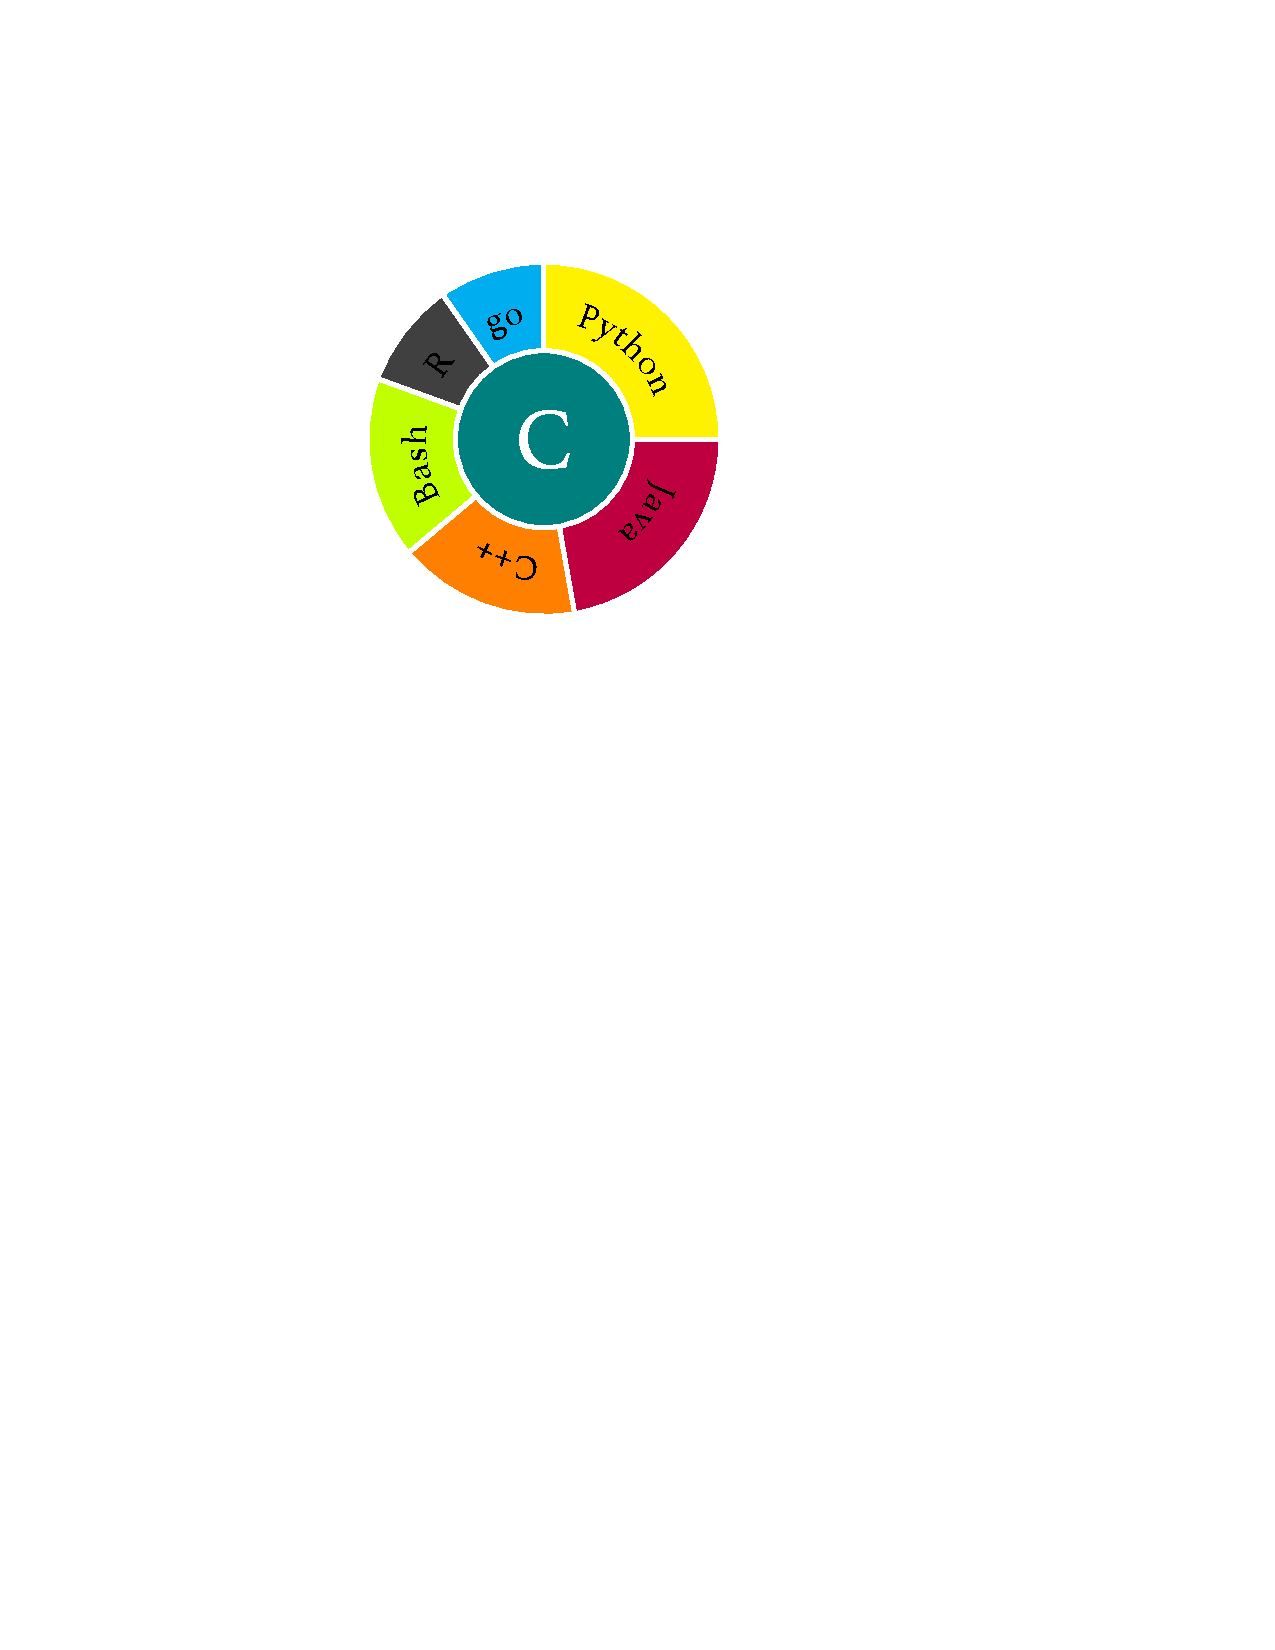
\includegraphics[scale=0.62]{img/programming.pdf}
    ~
  \section{\cuti 操作系统运维}
    \textbf{GNU/Linux}
\includegraphics[scale=0.16]{img/5stars}
    \textbf{MacOS}
\includegraphics[scale=0.16]{img/4stars}
    \textbf{Windows}
\includegraphics[scale=0.16]{img/2stars}
  \section{\cuti 其他技能}
    ~
    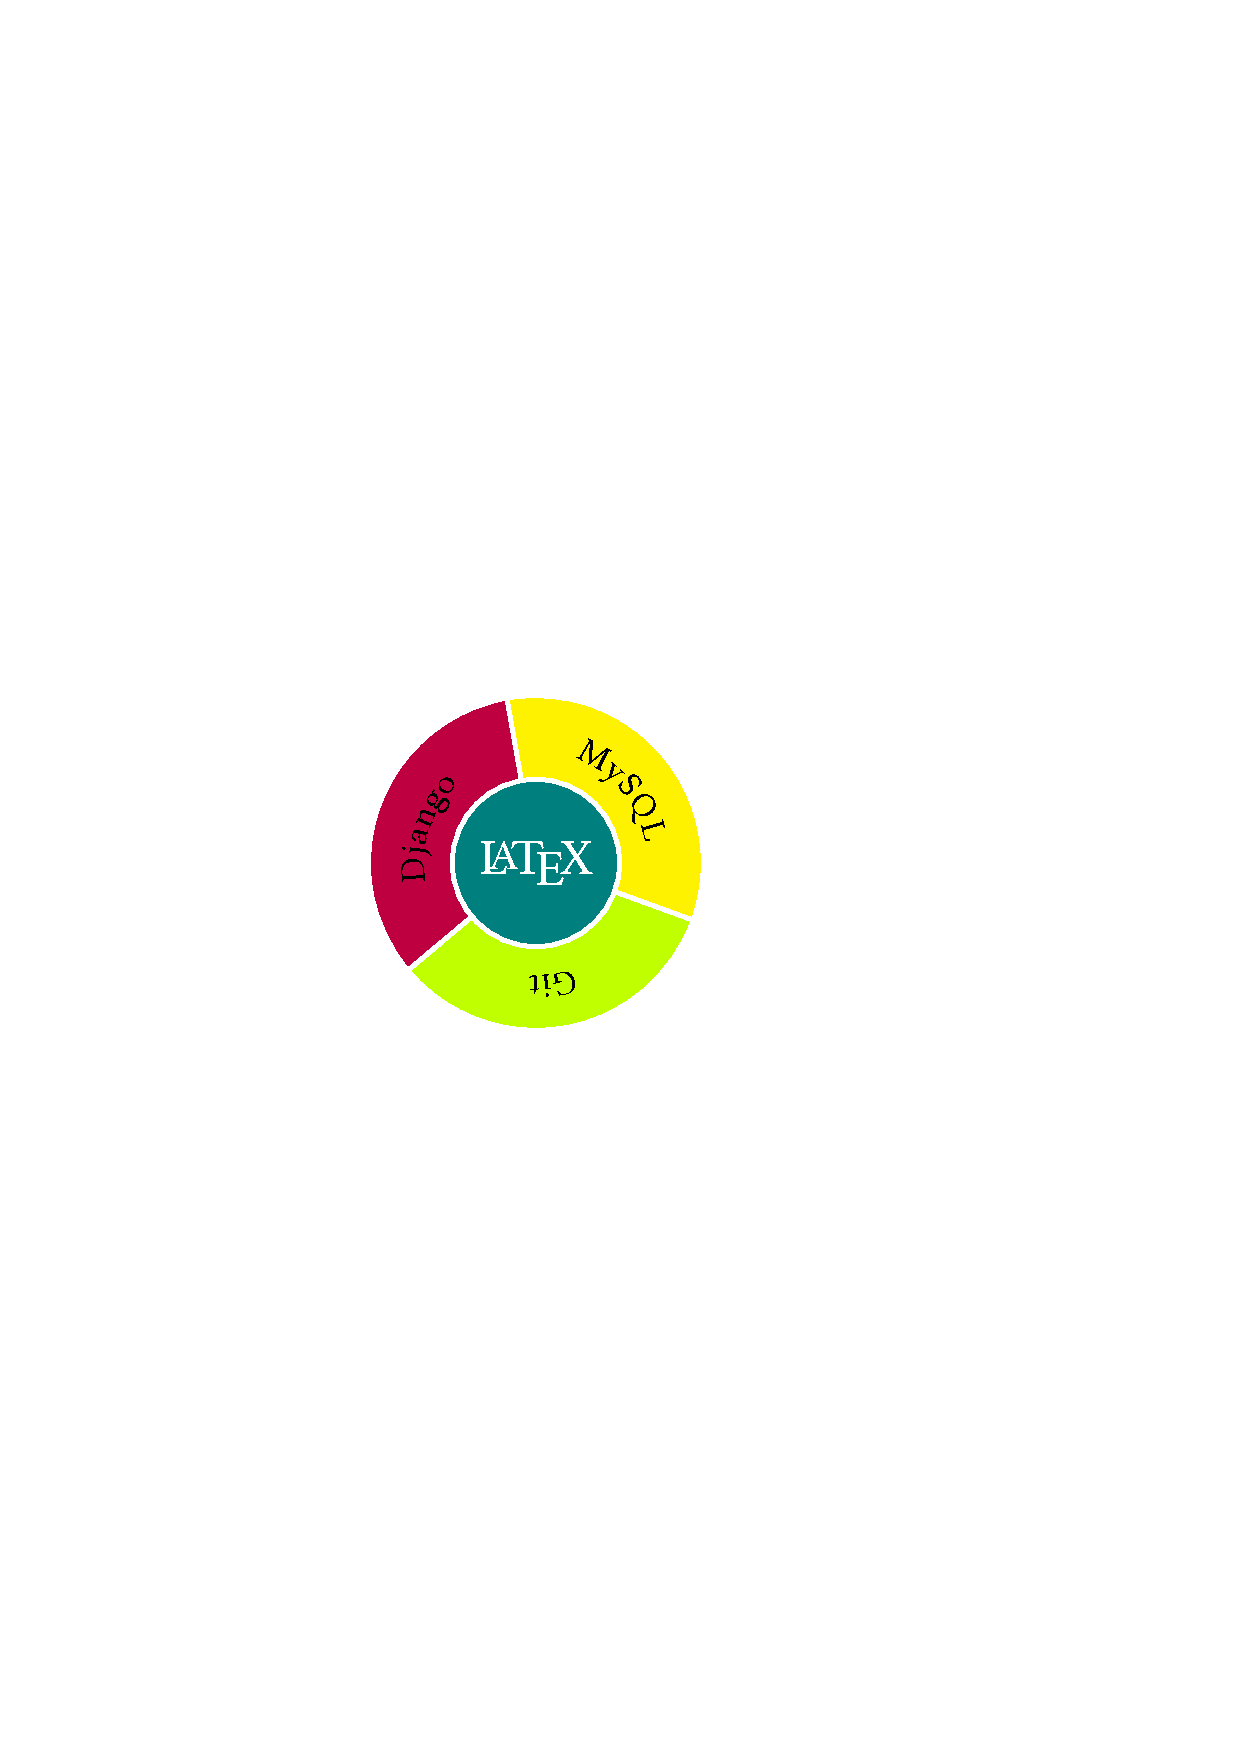
\includegraphics[scale=0.62]{img/personal.pdf}
    ~
  \section{\cuti 语言}
    \textbf{English}
\includegraphics[scale=0.16]{img/5stars}
    \textbf{日本語}
\includegraphics[scale=0.16]{img/2stars}
\end{aside}

\section{\cuti 重要项目经历}
\begin{entrylist}
  \entry
    {2013 - 2015}
    {\cuti 项目名称}
    {项目支持类型}
    {项目主要研究内容,死垃圾费拉时间的法律框架撒打飞机啊第三方就爱上来的发的是机房拉动是附近拉萨的福建师大立法水电费就撒旦了发的时间浪费第三方家里的事啊放假v\\}
  \entry
    {2012 - 2013}
    {\cuti 项目2名称}
    {自然科学基金}
    {研究虚拟机地方叫老大顺丰;拉萨的机房阿呆是家里附近大师李会计法电视剧方老师大家放假 大家阿里放假,打飞机。\\}
    \entry
    {2013 - 2014}
    {\cuti 项目3名称}
    {}
    {研究阿里的会计法律大家了;高杰拉德;水果就爱上的国家阿里山的结果了开发商打几个耳光隔绝了个。\\}
\end{entrylist}

\section{\cuti 高等教育经历}
\begin{entrylist}
  \entry
    {2012 - 2014}
    {\cuti 软件工程 硕士学位}
    {老鼠大学}
    {研究方向:xxxxxx\\
    参与竞赛:xxxxxxxxx\\
    骨干经历:xxxxxxxxx
\\}
  \entry
    {2008 - 2012}
    {\cuti 计算机科学与技术 学士学位}
    {老鼠大学}
    {主要方向:xxxxxxxxx\\
    参与竞赛:xxxxxxxxxx\\
    参与项目:xxxxxxxxxxx\\
    骨干经历:xxxxxxxxxxx\\
    其他:xxxxxxxx
  \\}
\end{entrylist}

\section{\cuti 论文发表情况}
\begin{entrylist}
  \entry
    {09/2014}
    {\cuti 论文名称,作者}
    {论文发布单位}
    {\emph{论文大概内容}}
\end{entrylist}\\

\section{\cuti 出版物发表情况}
作者\\
\textbf{书名}\\
\emph{主要工作}
\\

\vspace{40pt}

\begin{flushright}
\emph{二〇一四年六月三十日}
\end{flushright}
\begin{flushright}
\emph{大山鼠}
\end{flushright}

%%% This piece of code has been commented by Karol Kozioł due to biblatex errors. 
% 
%\printbibsection{article}{article in peer-reviewed journal}
%\begin{refsection}
%  \nocite{*}
%  \printbibliography[sorting=chronological, type=inproceedings, title={international peer-reviewed conferences/proceedings}, notkeyword={france}, heading=subbibliography]
%\end{refsection}
%\begin{refsection}
%  \nocite{*}
%  \printbibliography[sorting=chronological, type=inproceedings, title={local peer-reviewed conferences/proceedings}, keyword={france}, heading=subbibliography]
%\end{refsection}
%\printbibsection{misc}{other publications}
%\printbibsection{report}{research reports}

\end{document}
